% !TEX root = tesis.tex

\chapter{Detección de partículas energéticas\\ solares en el \emph{SciCRT}}
\chaptermark{Detección de partículas}
\label{chap:cuatro}
\section{Desempeño del \emph{SciCRT} como detector de RC}

\begin{figure}
        \centering
        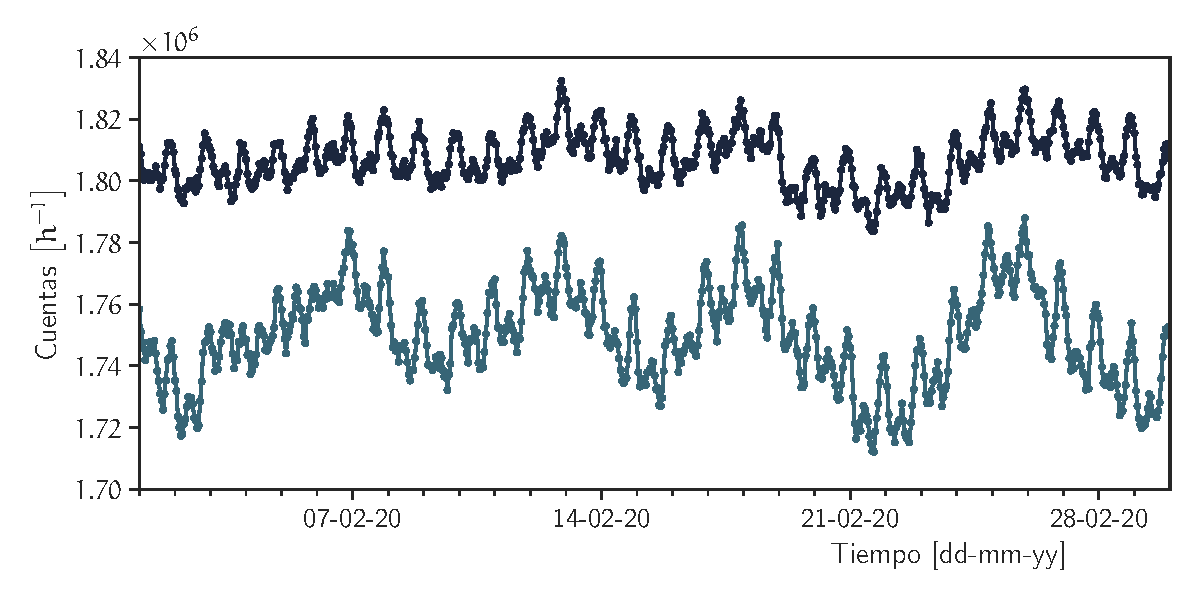
\includegraphics[width=\textwidth]{muon-monthly.pdf}
        \caption{Total de eventos de muones registrados durante Febrero \num{2020} por el SciCRT (linea azul oscura) en comparación con datos del NM de la Ciudad de México (línea azul claro).}
        \label{fig:muon-monthly}
\end{figure}

\begin{figure}
        \centering
        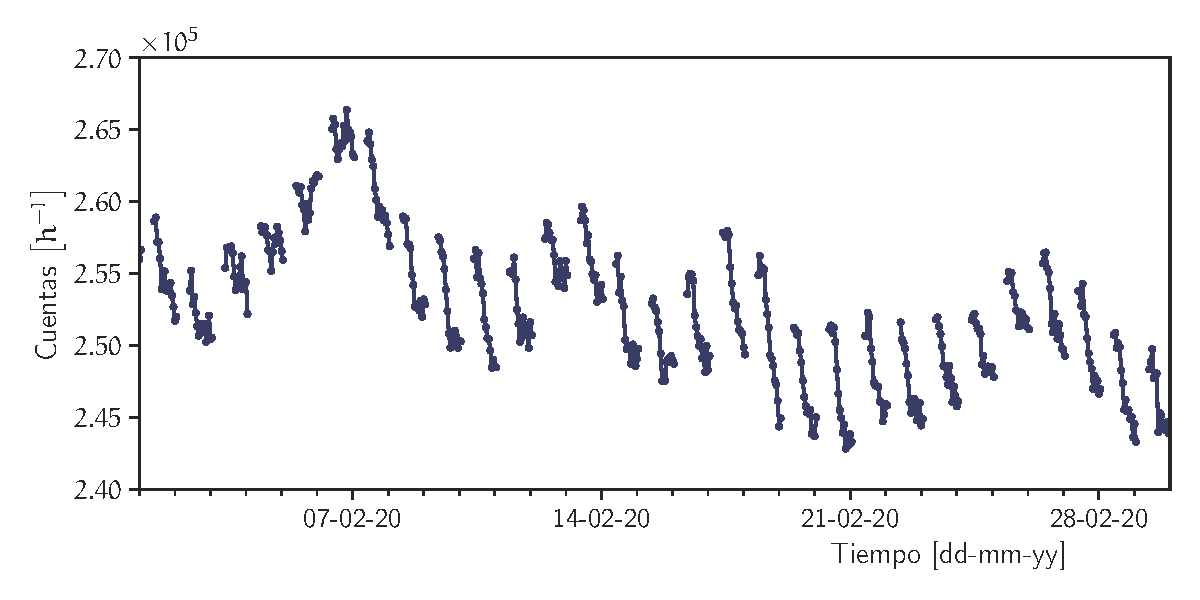
\includegraphics[width=\textwidth]{neutron-monthly.pdf}
        \caption{Total de eventos de partículas neutras registrados durante Febrero \num{2020} por el SciCRT (linea azul oscura) en comparación con datos del NM de la Ciudad de México (línea azul claro).}
        \label{fig:neutron-monthly}
\end{figure}

\begin{figure}
        \centering
        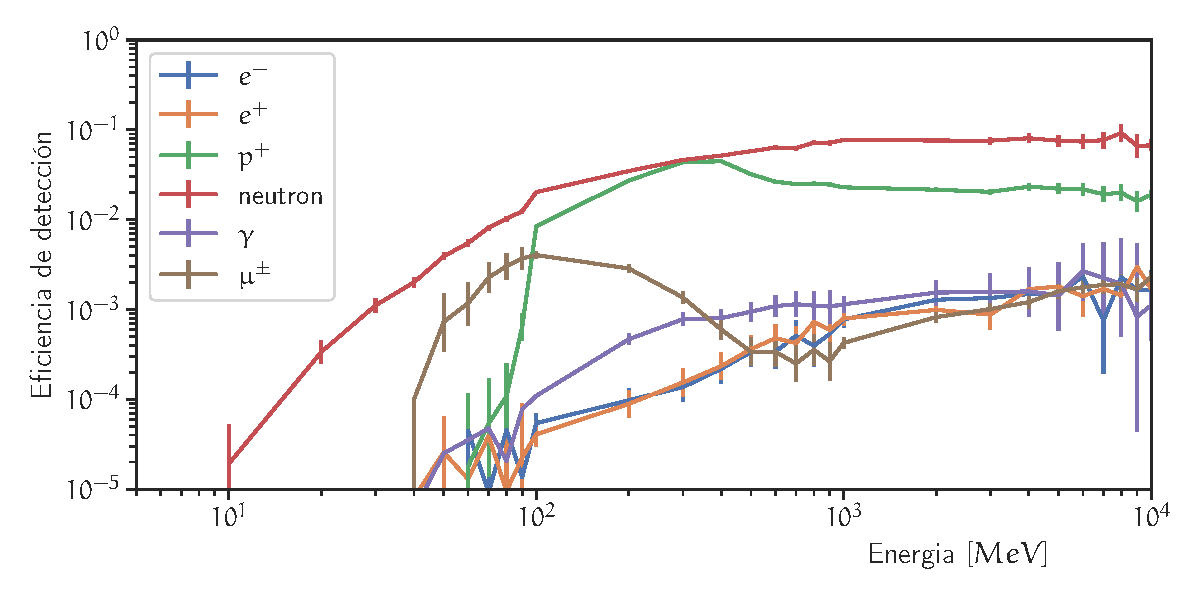
\includegraphics[width=\textwidth]{scibar-efficiency.pdf}
        \caption{Eficiencia de detección del SciCRT para diferentes especies de partículas en función de la energía incidente.}
        \label{fig:total-efficiency}
\end{figure}

\begin{figure}
        \centering
        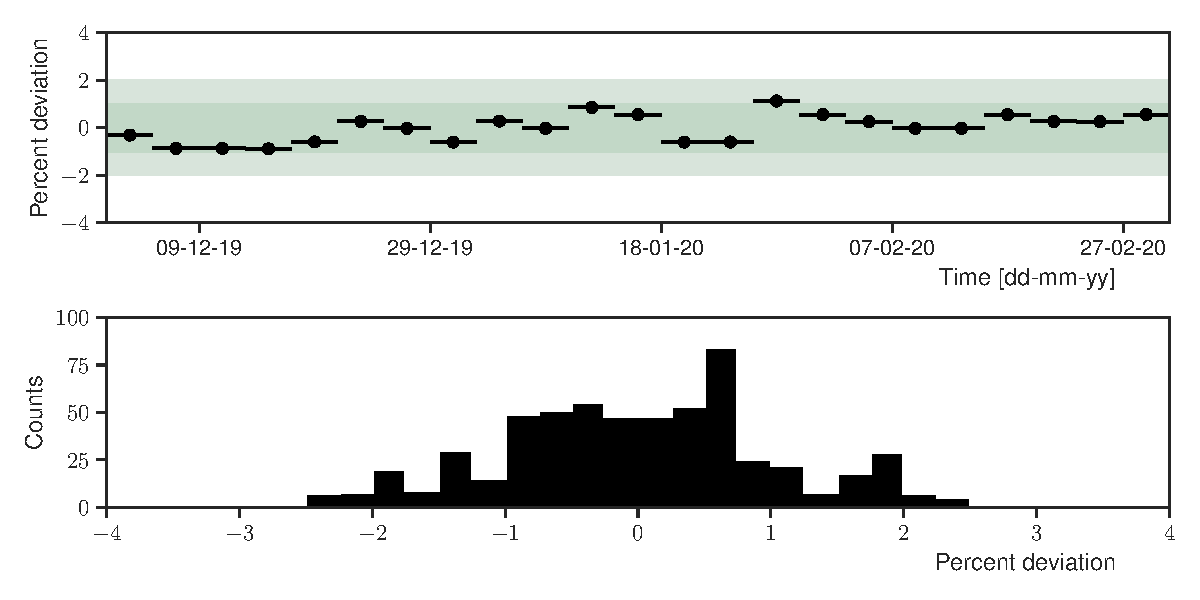
\includegraphics[width=\textwidth]{neutron-mip_stability.pdf}
        \caption{Estabilidad de la ganancia de los MAPMTs durante un periodo de tres meses. El panel superior muestra la variación en el tiempo de uno de los MAPMT. Las áreas sombreadas corresponden con las variaciones de \SI{\pm 1}{\percent} y \SI{\pm 2}{\percent}. El panel inferior es la distribución de todos los MAPMTs.}
        \label{fig:mip-stability}
\end{figure}



\begin{figure}
        \centering
        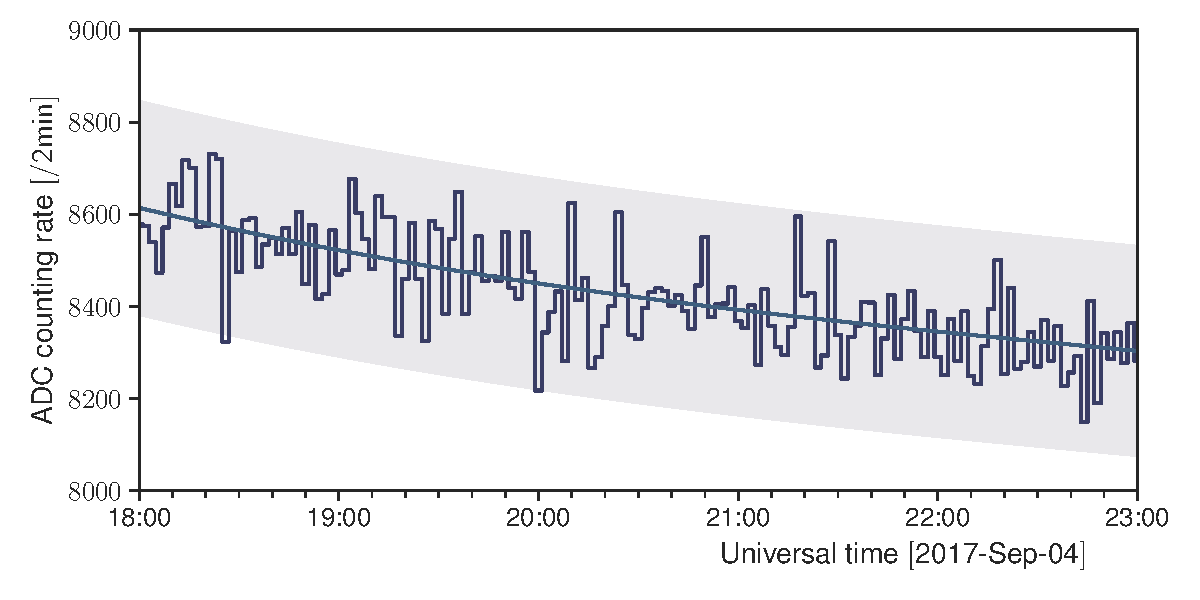
\includegraphics[width=\textwidth]{neutron-170904.pdf}
        \caption{Perfil temporal de eventos registrados por el \emph{SciCRT} el \num{4} de Septiembre de \num{2017}. El área sombreada representa el nivel de $3.0\sigma$.}
        \label{fig:september-04}
\end{figure}

\begin{figure}
        \centering
        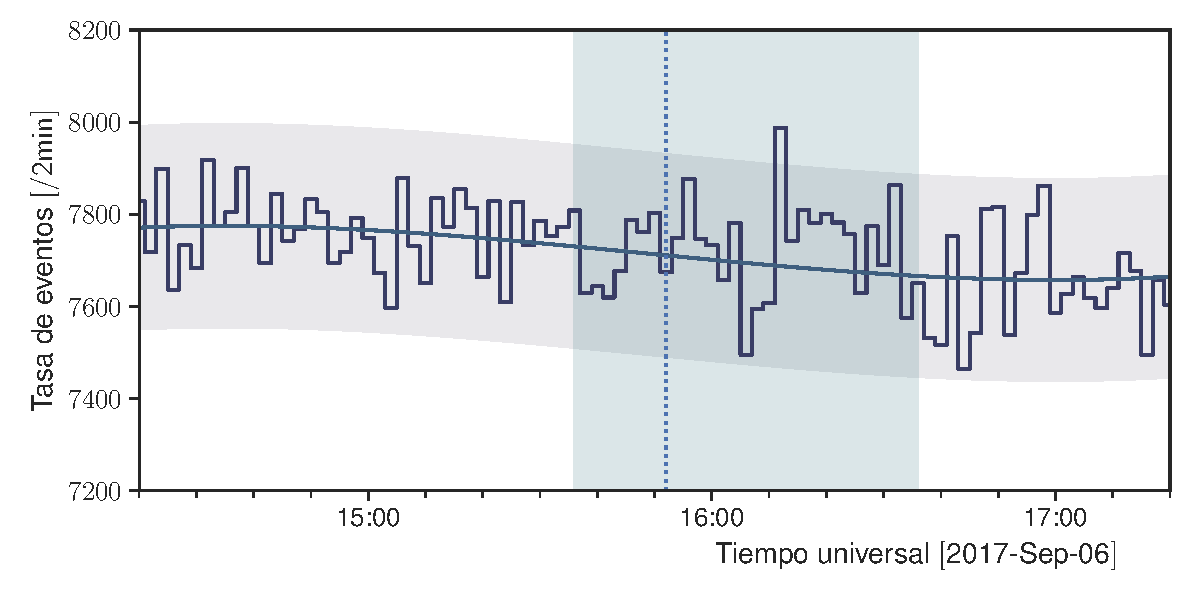
\includegraphics[width=\textwidth]{neutron-170906.pdf}
        \caption{Perfil temporal de eventos registrados por el \emph{SciCRT} el \num{4} de Septiembre de \num{2017}. El área sombreada representa el nivel de $3.0\sigma$..}
        \label{fig:september-06}
\end{figure}
